%!TEX program = <xelatex>
\documentclass{pracamgr}
\usepackage{mystyle}
\usepackage{classDetails}

\begin{document}

	\setcounter{page}{1}
	\pagenumbering{roman}

	\maketitle
%\renewcommand\bibname{Spis literatury}	
	
	\begin{abstract}
Parallel Tempering (PT) is an extension to standard Metropolis-Hastings (MH) algorithm for simulating samples from a given distribution. The standard MH algorithm with high probability remains a local algorithm, in the sense that samples are drawn from some local probability mass cluster. This is highly problematic in case of multimodial distributions that frequently appear in applications, i.e. in bayesian hierarchical models. The PT algorithm is one of most celebrated possible solutions to that problem. 

Here we present a newly developed template for running simulations written in the R statistical programming language. Being highly modular it provides a general tool for performing simulations with many user provided state-spaces.
\end{abstract}

	\tableofcontents
	
	\addcontentsline{toc}{section}{List of figures}
	\listoffigures

	\addcontentsline{toc}{section}{List of tables}
	\listoftables

	\setcounter{page}{1}
	\pagenumbering{arabic}

	% Chapter
		% Section
		% Section
		% ...

	\chapter*{Introduction}
		\include*{./tex/introduction}
		
	\chapter{ Motivation }\label{motivation}	
		\include*{./tex/motivation/motivation}	
	
	\chapter{ Theory }\label{theory}	
		\include*{./tex/theory/theory}
	
	\include*{./tex/implementation/implementation}
		\include*{./tex/implementation/divisionIntoObjects}
		\include*{./tex/implementation/methodsAndFunctions}
		\include*{./tex/implementation/kolmogorovSmirnov}

	\include*{./tex/simulationsResults/simulationsResults}
	\include*{./tex/summary}

	\begin{appendices}
		\include*{./tex/appendices/methodsDescribed}
	\end{appendices}	

	\bibliographystyle{./bibliography/eccaNoNotes}
	% \bibliography{./bibliography/myBooks}
	\bibliography{myBooks}

\end{document}






%%% Przydatne

\begin{figure}
	\begin{minipage}[b]{.5\linewidth}
		\centering 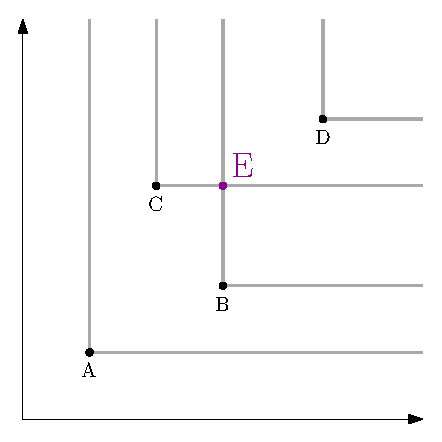
\includegraphics[scale=1]{./img/KS1.eps}
		\subcaption{Sample points and level sets of an examplary \ecdf.}\label{simpleEcdf}
	\end{minipage}%
	\begin{minipage}[b]{.5\linewidth}
		\centering 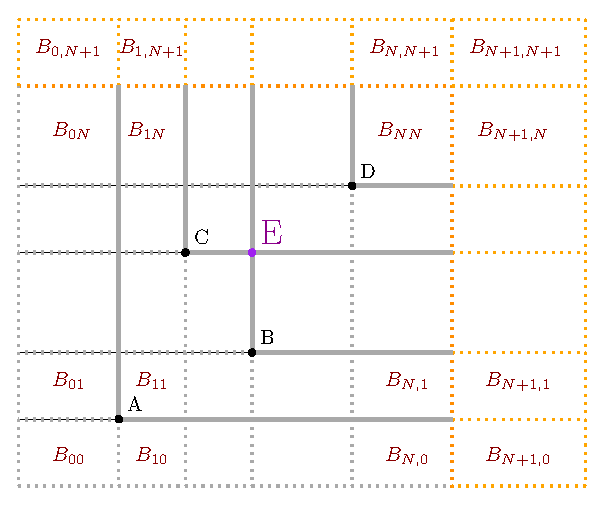
\includegraphics[scale=1]{./img/KS2.eps}
	\subcaption{Division of the state-space.}\label{fig:1b}
	\end{minipage}
	\caption{Calculations of the KS-distance.}\label{fig:1}
\end{figure}
s
The applicability of the PT algorithm in molecular biology stems mostly from the ever growing interest in the Bayesian inference. The mixture models for instance have been applied in the identification of gene co-expression patterns in microarray data. With the spread of use of such methods, the PT algorithm gains of importance.